\documentclass[pdftex,12pt,a4paper]{report}

\usepackage[portuguese,english]{babel}
\usepackage[T1]{fontenc} 
\usepackage[utf8]{inputenc}
\usepackage[pdftex]{graphicx}
\usepackage{minitoc}
\usepackage{hyperref}
\usepackage{indentfirst}
\usepackage[compact]{titlesec}
\usepackage{fancyhdr}
\usepackage{caption}
\usepackage{pgfplots}
\usepackage{pgfplotstable}
\usepackage{fixltx2e}
\usepackage{mathtools}
\usepackage{fancyhdr}

\pagestyle{fancy}
\renewcommand*\thesection{\thechapter\arabic{section}}
\newcommand{\HRule}{\rule{\linewidth}{0.5mm}}
\begin{document}

\begin{titlepage}

\begin{center}


\includegraphics[width=0.15\textwidth]{./logo}\\[0.5cm]    

\textsc{\large Universidade de Aveiro \\[1cm]\large departamento de electrónica, telecomunicações e informática}\\[1cm]

\textsc{\large{42532}\large - Base de Dados \\[1cm]}

\HRule \\[0.5cm]
{ \huge \bfseries Football Club}\\[0.4cm]
{ \large \bfseries Trabalho Prático Final}\\[0.4cm]
\HRule \\[1cm]

\textsc{\small{8240 - MESTRADO INTEGRADO EM ENGENHARIA DE COMPUTADORES E TELEMÁTICA}}\\[1cm]

\begin{minipage}{0.4\textwidth}

\begin{flushleft} \large
\href{mailto:rafael.ferreira@ua.pt}{António Rafael da \\ Costa Ferreira }
 \small{\\NMec: 67405 | P4G5}
\end{flushleft}
\end{minipage}
\begin{minipage}{0.4\textwidth}

\begin{flushright} \large
\href{mailto:rodrigocunha@ua.pt}{Rodrigo Lopes \\ da Cunha}
\small{\\NMec: 67800 | P4G5}
\end{flushright}
\end{minipage}\\[1cm]

{\large Docente: Carlos Manuel Azevedo Costa   }\\[0.5cm]

\vfill

{\large Junho de 2015 \\ 2014-2015}

\end{center}

\end{titlepage} %Titulo do Relatorio
\renewcommand{\headrulewidth}{0pt}

%Cabeçalhos de rodapé
\fancyhead{}
\fancyfoot{}
\lhead{Football Club - Trabalho Prático Final}
\rhead{BD - 2014/2015}
\lfoot{\textit{P4G5} \\ Rafael Ferreira nmec: 67405 \\ Rodrigo Cunha nmec: 67800}
\rfoot{\thepage}

%Renomear Comandos
\renewcommand*\contentsname{Conteúdos}
\renewcommand*\figurename{Figura}
\renewcommand*\tablename{Tabela}

%Conteúdos, dar paragrafo
\tableofcontents
%Headers
\renewcommand{\headrulewidth}{0.15pt}
\renewcommand{\thechapter}{}

\clearpage

\section{Introdução}
% o que, porquê e o objetivo
O trabalho proposto para o projeto da unidade curricular de Base de Dados é uma plataforma de gestão de um clube de futebol. Usando os conhecimentos adquiridos, propôs-se o desenvolvimento deste projeto visto que o futebol é uma modalidade mundial, envolvendo vários tipos de interesse. 

O objetivo desta base de dados desenvolvida é permitir a gestão de todos os processos de um clube de futebol, como será visto mais à frente.

Além de se ter desenvolvido esta base de dados, desenvolveu-se uma aplicação WPF C\# para permitir a manipulação dos dados da base de dados de forma mais simplificada para um utilizador final.

Esta base de dados deve fornecer ferramentas que permitam a criação, remoção, alteração e consulta da base de dados de forma segura, eficiente e robusta.

O relatório reflete todos os passos e decisões tomadas na criação da base de dados que sustenta o projeto bem como uma descrição das capacidades da aplicação desenvolvida para o cliente.

Para a criação deste projeto foi seguido o processo leccionado nas aulas, sendo estas as seguintes fases do processo: análise de requisitos, desenho conceptual, desenho do esquema lógico, desenho do esquema físico e administração.

\newpage
\section{Análise de Requisitos}

A análise de requisitos foi uma das partes mais importantes do processo de concepção do projeto uma vez que ajudou a ter uma visão clara do que o sistema teria de suportar. Após realizado um "brainstorming", estas são as características que o sistema deve suportar:

Uma \textbf{pessoa} é identificada por um nome, B.I. (sendo que este B.I. é único), endereço, NIF, Sexo, Data de Nascimento e Nacionalidade. Esta pessoa pode ser uma Pessoa que pertença ao pessoal interno do clube (Staff) ou ser sócio do clube. 

Uma \textbf{pessoa interna} ao clube tem salário e um ID que é automaticamente atribuído e o identifica dentro do clube.

Um \textbf{sócio do clube} tem um nº de sócio, o ano até que as suas cotas estão pagas (são cotas anuais) e um valor de cotas que tem de pagar todos os anos. Um sócio pode ter ou não um \textbf{lugar anual}, tendo este, um valor, data de início, duração, Nº Lugar e Nº Fila e ID da secção.

Um \textbf{lugar} tem um nº de lugar e fila. Uma \textbf{secção} tem um ID de secção e tipo. 

Um \textbf{jogador} é uma pessoa interna ao clube e é identificado com um ID da federação, peso e altura. Este joga em equipas do clube.

Um \textbf{treinador} é uma pessoa interna do clube e é identificado com um ID da federação e cargo. Este tem equipas do clube.

Uma \textbf{equipa} tem uma idade máxima de jogadores que podem pertencer à mesma e um nome único.

Uma equipa pode ter \textbf{treinos} que são caracterizados por uma data e uma hora e são realizados num determinado campo.

Um \textbf{campo} tem um endereço e um ID.

Uma pessoa interna ao clube (\textbf{Staff}) tem um cargo e pode trabalhar um Departamento.

Um \textbf{departamento} tem um endereço, ID de departamento e um nome.

\newpage

Foram também registadas algumas especificações para o desenho conceptual:

- Uma pessoa pode ser um sócio e uma pessoa interna.

- Uma pessoa interna ao clube pode ser um jogador, um coach ou um membro do staff.

- Um sócio pode ter vários lugares anuais mas um lugar anual apenas pertence a um membro.

- Um lugar pode ter vários lugares anuais mas um lugar anual apenas tem um lugar.

- Uma secção pode ter vários lugares mas um lugar pode ter apenas uma secção.

- Um membro do staff apenas pode trabalhar num departamento e um departamento pode ter vários membros do staff.

- Um jogador pode jogar em várias equipas e uma equipa pode ter vários jogadores.

- Um treinador pode jogar em várias equipas e uma equipa pode ter vários treinadores.

- Uma equipa pode ter vários treinos mas um treino apenas pode ter uma equipa.

- Um treino apenas pode ter um campo e um campo pode ter vários treinos.

\newpage
\section{Diagrama entidade relação}
Depois da análise de requisitos desenhou-se o diagrama entidade relação do nosso sistema. Este desenho foi descrito através de um diagrama ER\ref{fig:eer}. No diagrama, foram definidas entidades, atributos, relações, cardinalidades e dependências.

\begin{figure}[!htb]
 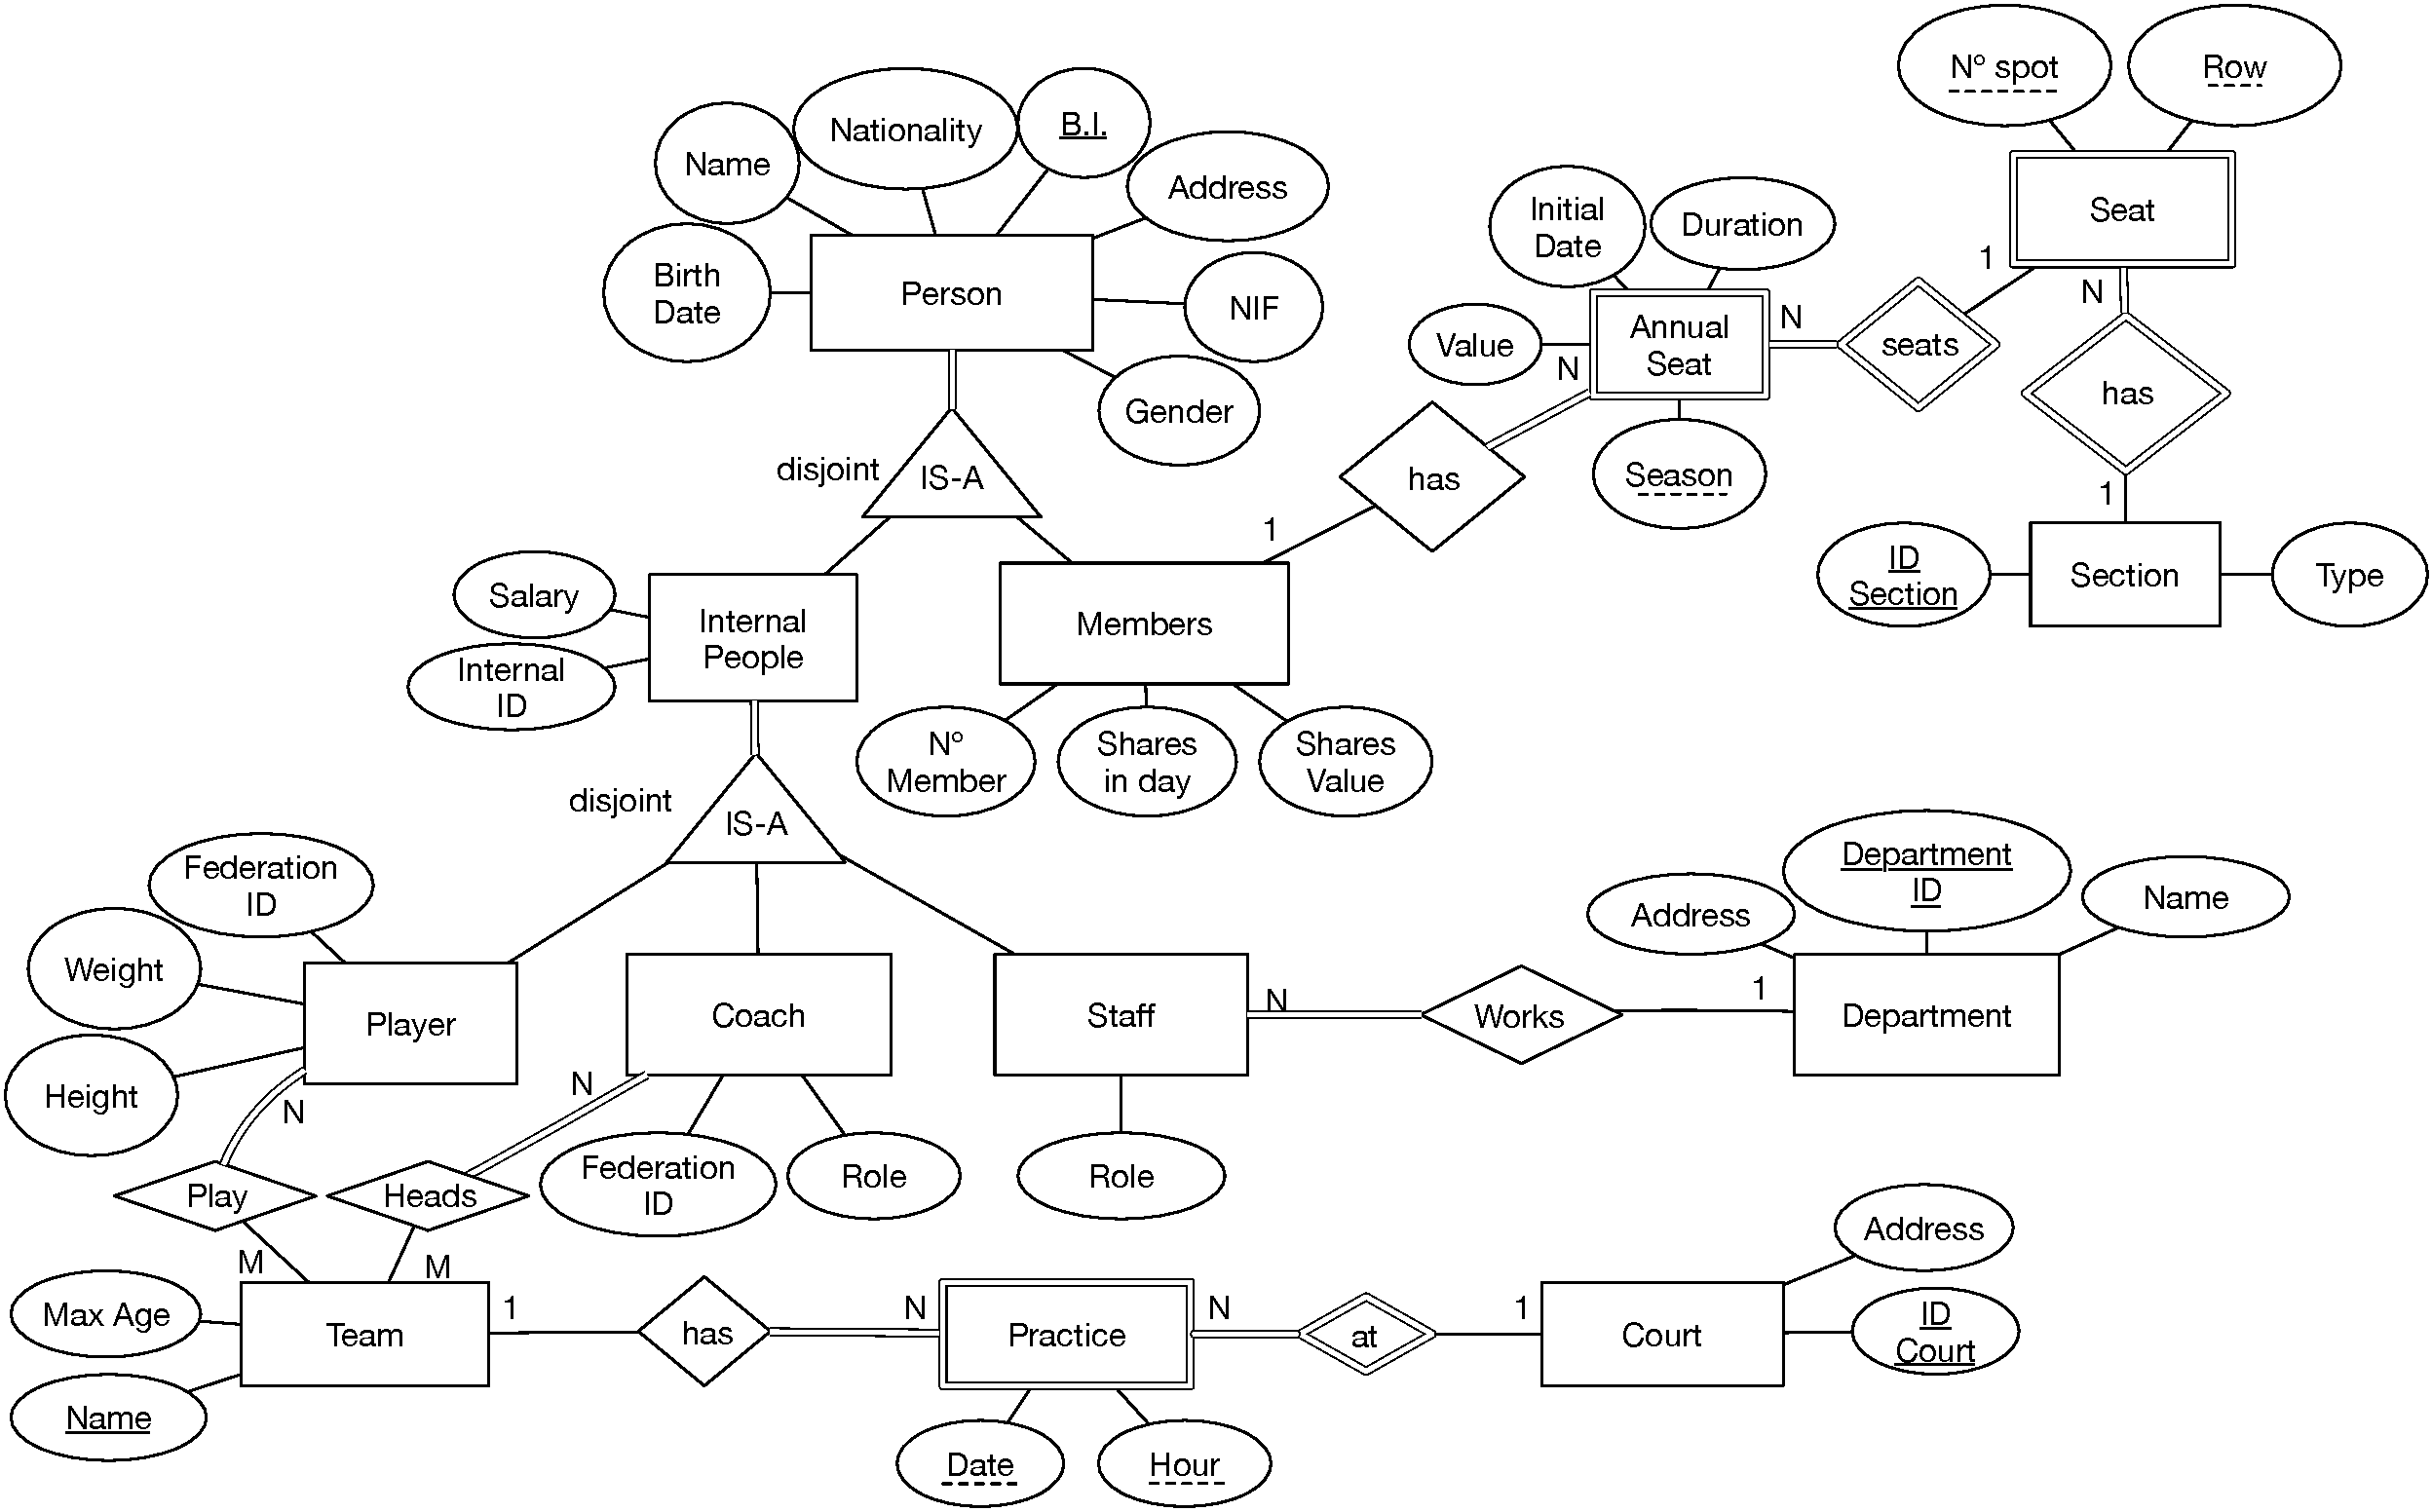
\includegraphics[width=135mm,scale=1]{EER.pdf}
 \caption{\\Diagrama entidade relação}\label{fig:eer}
\end{figure}

As entidades e os seus atributos correspondem à análise de requisitos realizada anteriormente. As relações são todas binárias.

\newpage
\section{Esquema Relacional da BD}
Após a construção do nosso desenho conceptual procedeu-se à elaboração do Modelo Relacional. Este modelo foi construído tendo por base o diagrama entidade relação e as regras para a realização desta tarefa. Cada entidade e cada relação irá gerar uma única tabela e após realizados os passos para conversão do desenho conceptual no modelo relacional 
foi criado o modelo relacional\ref{fig:mr}.

\begin{figure}[!htb]
 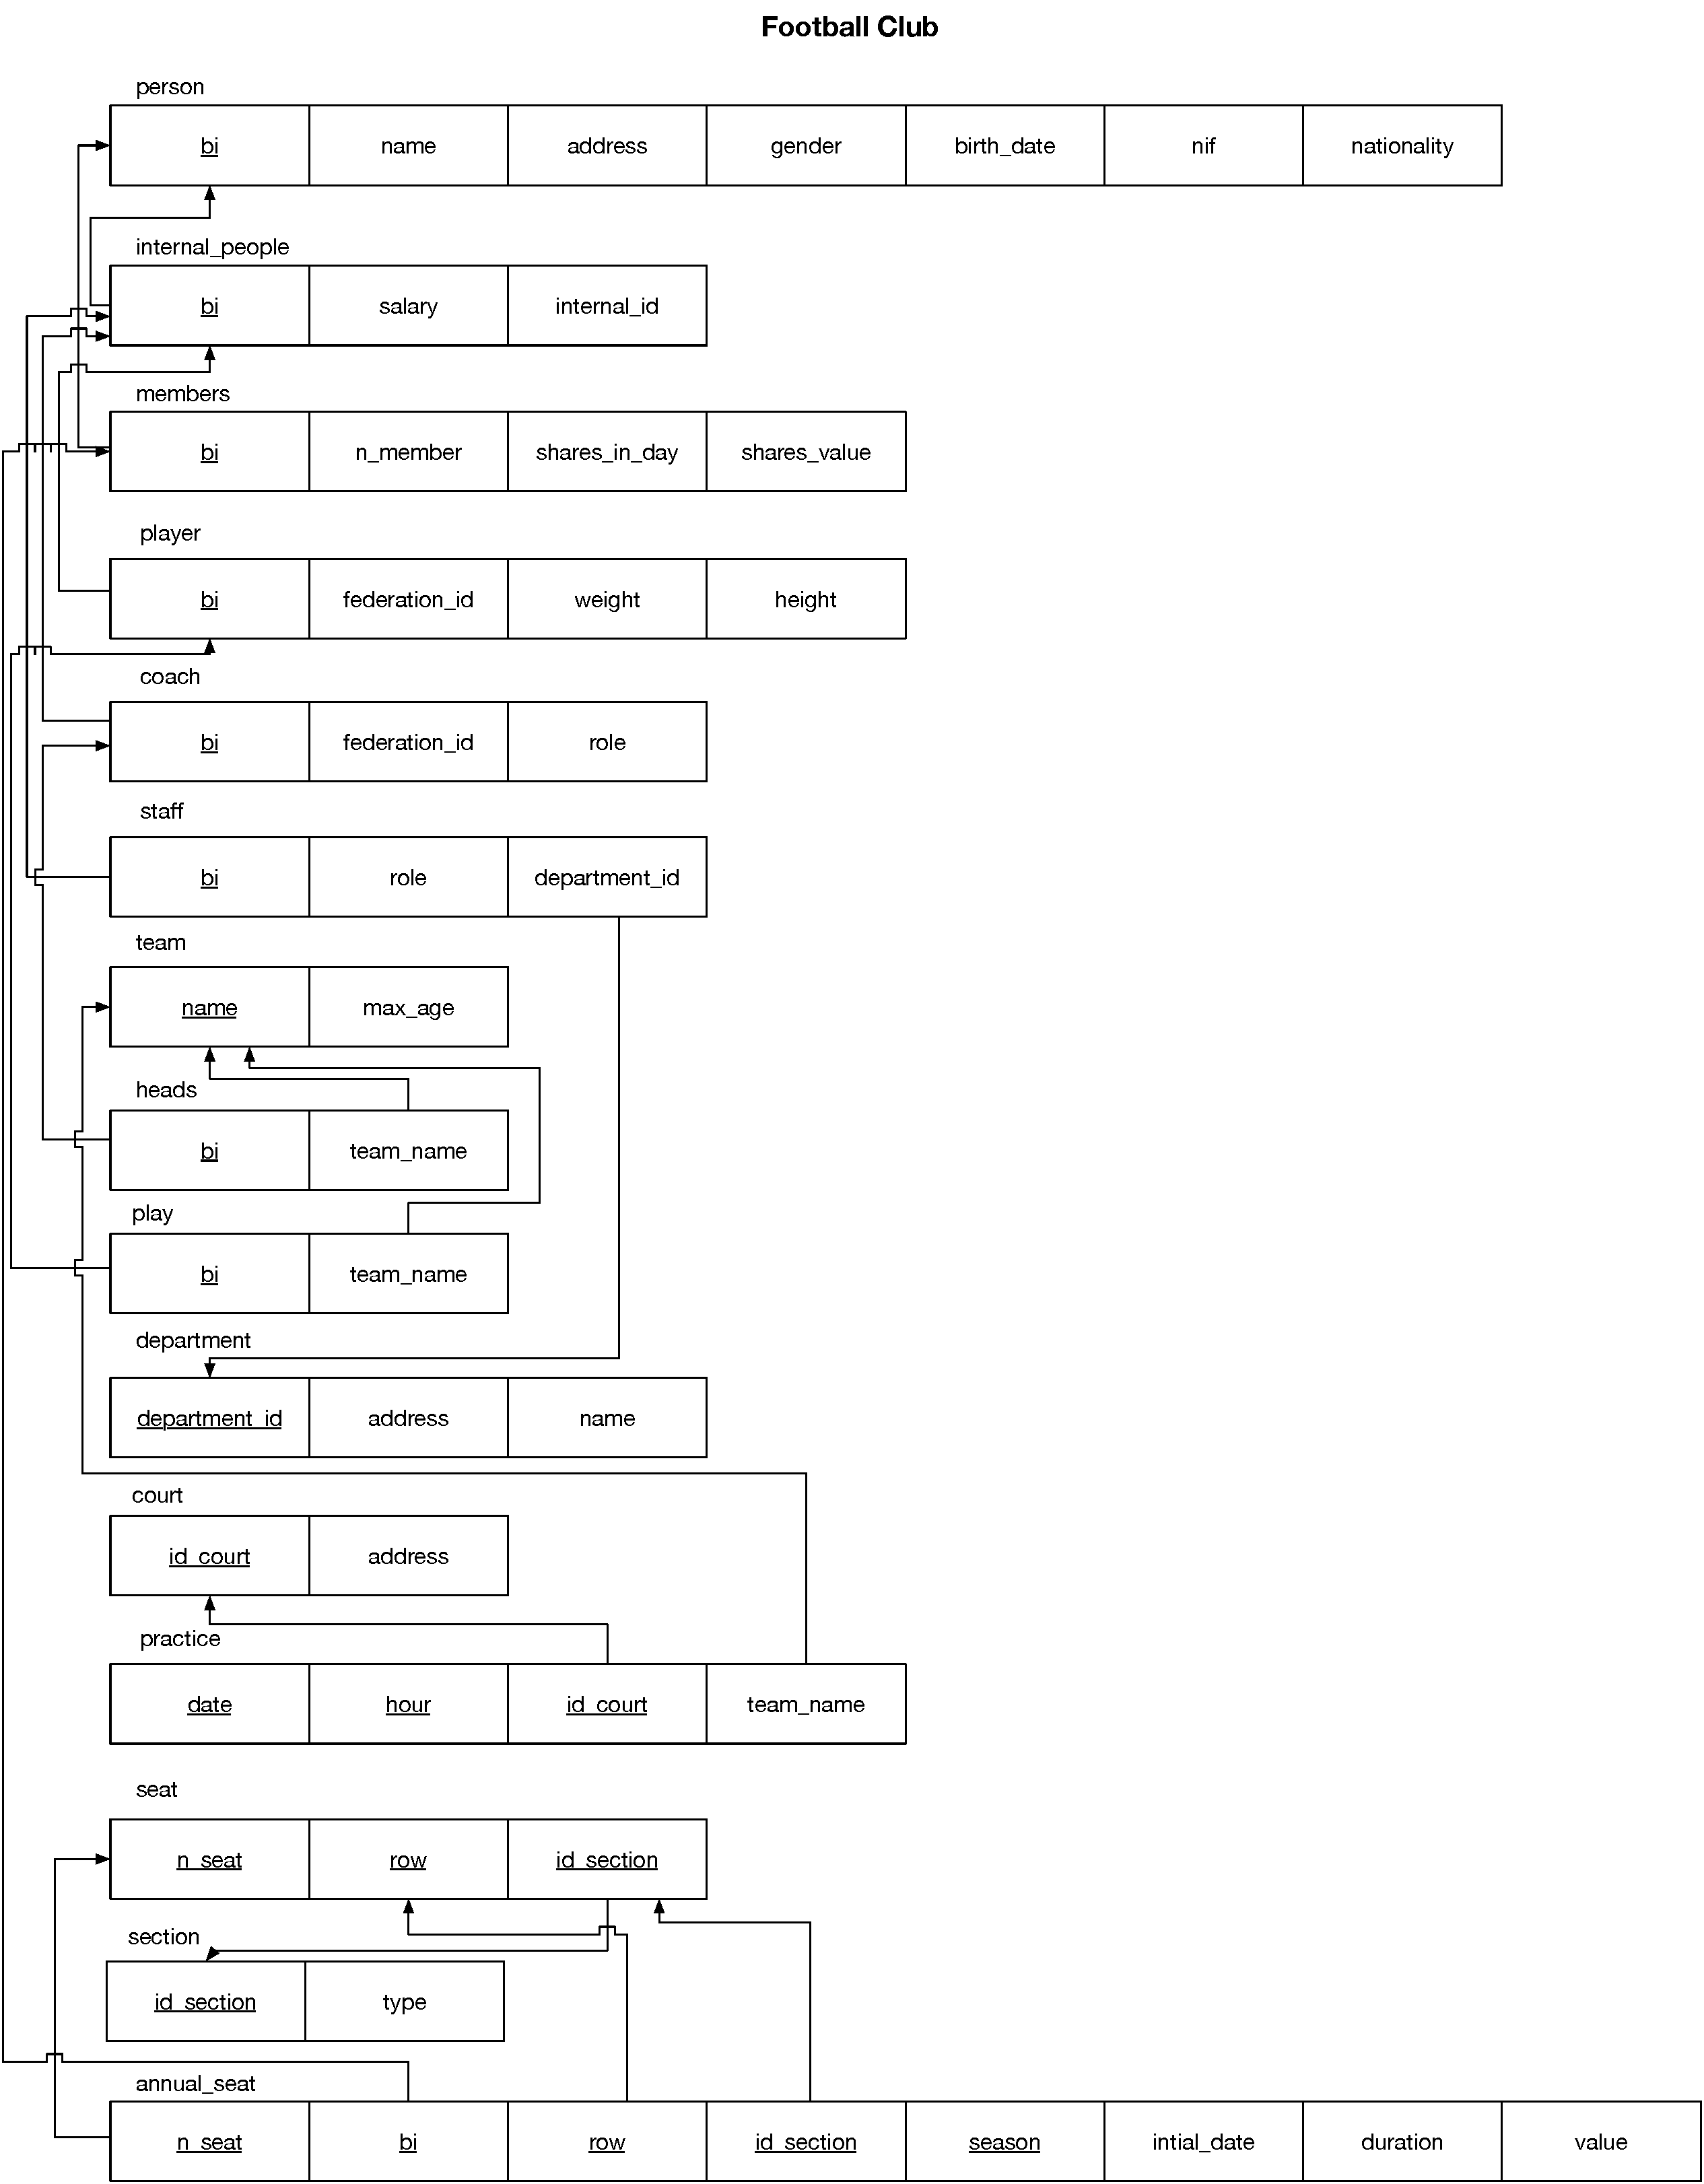
\includegraphics[width=100mm,scale=1]{modelo_relacional.pdf}
 \caption{\\Modelo relacional}\label{fig:mr}
\end{figure}

\newpage
\section{Normalização}


\end{document}